\chapter{Introduction}
    %\addcontentsline{toc}{chapter}{\protect\numberline{}Introduction}
    
     % Might be useful: http://www.emerson.emory.edu/services/latex/latex_162.html

\section{General context}

%Since its early days, humankind has always felt the desire to fly. 

%It was not until the World War I, when planes took a fundamental role in the last stages of the 

%In World War I, airplanes played a fundamental role 


In the 20th century, the field of aeronautics has experimented a hectic growth since World War I (1914 - 1919), when airplanes played a fundamental role in the aerial battles. The advances in military aviation led to the apparition of the first airlines and the birth of commercial aviation after the war. It was not, however, until World War II (1939 - 1945) that the biggest progresses were made: technological improvements resulted in larger, more efficient aircrafts that were used for surveillance, in air battles or for bombing purposes. After this period, airplanes used during the war were recycled with civil purposes to transport cargo and passengers. This supposed the beginning of a new era for commercial aviation that has not stopped to grow until nowadays, where air transportation is an essential activity in today's society.

The increasing relevance of commercial aviation has been possible due to advances in aeronautical technologies, from structures and control systems to propulsion systems. In the case of the latter, the birth of the jet engine in the 1930s supposed a milestone that marked the transition from propelled airplanes working with internal combustion engines to faster ones powered by gas turbines. Improvements in propulsion technologies have led to bigger, more efficient engines which can produce more power in order to drive bigger airplanes faster during longer times, hence covering longer distances. 

%However, despite today's propulsion technologies being more efficient than those from its origins, they are not extent of pollutant emissions. The increasing demand of commercial transportation in the last years, as well as the increasing general concern for the effects of greenhouse gases on climate change, has made the aeronautical engine manufactures to place emissions' reduction as a major constraint for engine design. In this respect, pollutant species such as CO, CO$_2$ and NO$_\mathrm{x}$, generated during the combustion process, are meant to be reduced. 

However, despite today's propulsion technologies being more efficient than those from its origins, they are not extent of producing emissions. Species generated during the combustion process in gas turbines include CO$_2$, a greenhouse gas contributing to global warming, and CO and NO$_\mathrm{x}$, considered as pollutant emissions. In this respect, the increasing demand of commercial transportation and a rising general concern about the effects of climate change, have placed the need of reducing emissions, as well as noise, as a major constraint for the development of aviation in the decades to come. The Advisory Council of Aeronautic Research in Europe (ACARE) has settled the goal to reduce the emissions per passenger/kilometre of CO$_2$ by 75 $\%$ and of NO$_\mathrm{x}$ by 90 $\%$ for the year 2050 with respect to the levels of 2000 \citepColor[acare_strategic_2017].

Emissions of NO$_\mathrm{x}$ are a big concern due to their harmful effect in health and environment (e.g. it is one of the main species producing acid rain). The evolution of aeronautical engines in the last decades have led to higher combustion temperatures and larger Overall Pressure Ratios (OPR), which help to reduce fuel consumption but increase the production of NO$_\mathrm{x}$. Engine manufacturers have worked on mitigating this increasing trend, as shown by the evolution of NO$_x$ emissions with OPR for several generations of engines in Figure \ref{fig:NOX_emissions_with_OPR}. It is shown how certified engines have succeeded in reducing emissions below the ICAO-CAEP regulatory limits. Nevertheless, the NO$_\mathrm{x}$ are still expected to grow due to the expanding aerial traffic demand. Figure \ref{fig:NOX_forecasts} displays the forecasts for several traffic scenarios, where it is shown the potential effect of technology advances in the emissions at 2040 (lower bounds) with respect to the case where current technologies (of year 2017) would be used (upper bounds). Therefore, in order to maintain the emissions below a certain level and hence accomplish the ACARE goals, substantial efforts need to be done. One way of achieving this is by controlling and improving the combustion process, since it is known that NO$_\mathrm{x}$ are produced at high temperatures. For this purpose, the aeronautical community is working towards new combustion chambers and injection processes aiming at creating \textbf{lean combustion}.

\begin{figure}[h!]
	\centering
	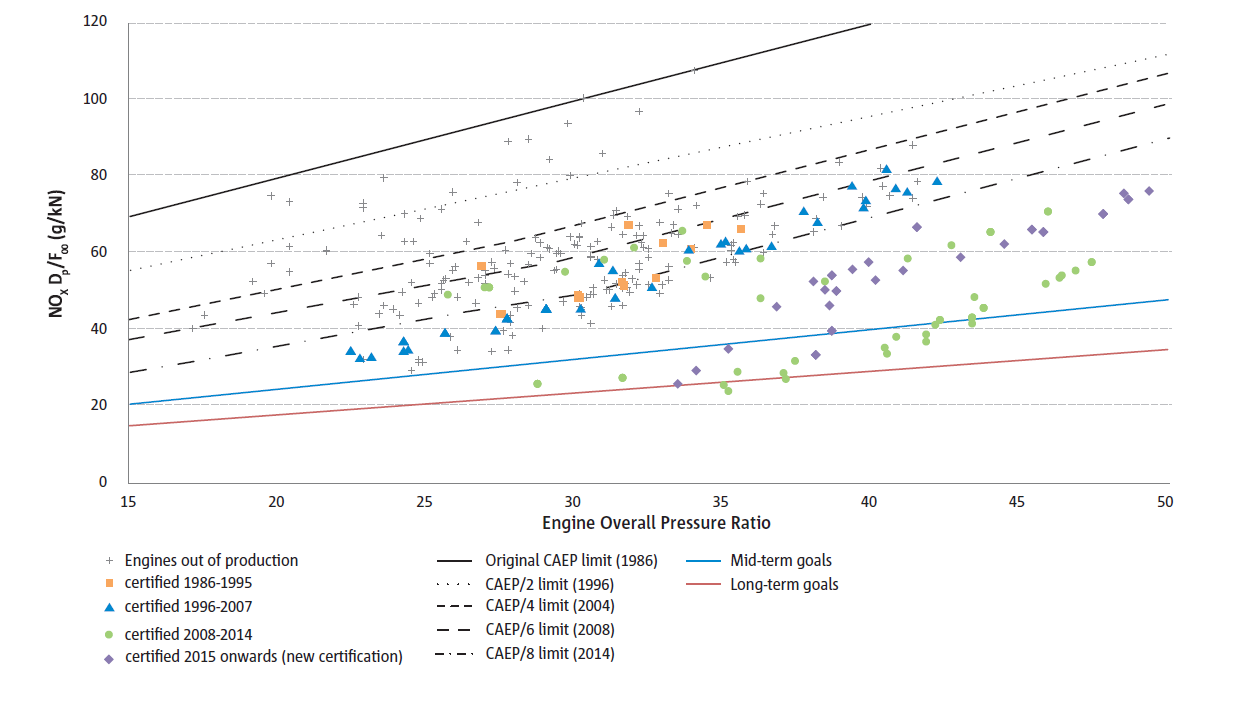
\includegraphics[scale=0.6]{./part0_intro/NOx_emissions_with_OPR}
	\caption{Evolution of NO$_x$ emissions with several generations of aircraft engines. Source: \citepColor[easa_european_2019]}
	\label{fig:NOX_emissions_with_OPR}
\end{figure}

\begin{figure}[h!]
	\centering
	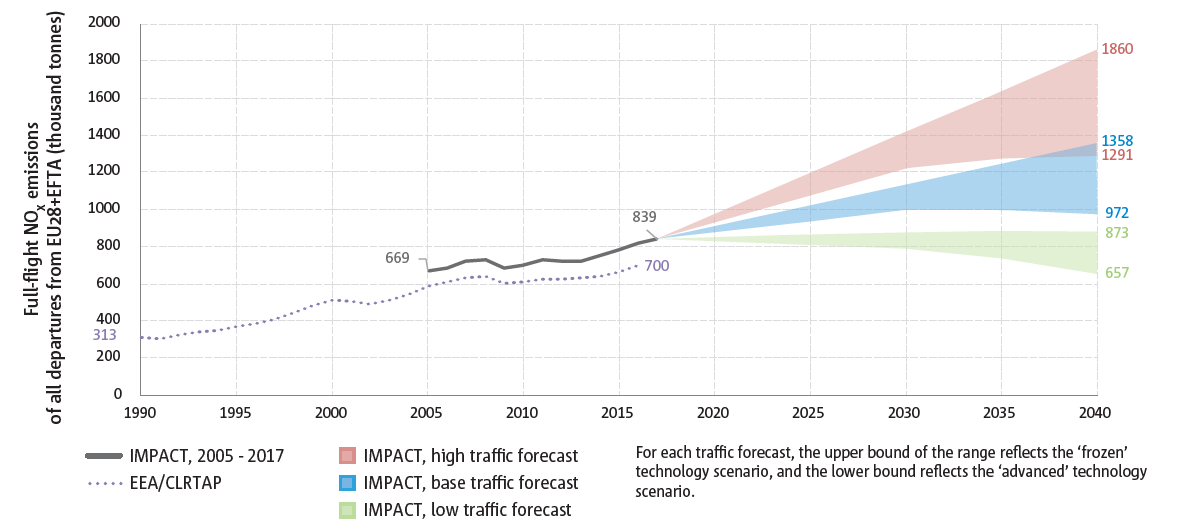
\includegraphics[scale=0.6]{./part0_intro/NOx_emissions_forecast_report2019}
	\caption{NO$_x$ emission forecasts from 2017 to 2040. Source: \citepColor[easa_european_2019]}
	\label{fig:NOX_forecasts}
\end{figure}


\section{Lean combustion in aeronautical gas turbines}

%Conventional combustors used to introduce only a small portion of air ($\sim 30 \%$ ) with the liquid injection system, and the rest was introduced through secondary holes located downstream (see Figure \ref{fig:combustor_conventional}). As a consequence, com

%\begin{figure}[h!]
%	\centering
%	\includegraphics[scale=0.6]{./part0_intro/combustor_conventional}
%	\caption{Conventional combustor. Source: \citeColor[lefebvre_gas_2010].}
%	\label{fig:combustor_conventional}
%\end{figure}

With the objective of reducing NO$_\mathrm{x}$ emissions in aeronautical combustion chambers, the community has worked towards the implementation of concepts aiming at producing lean combustion. The motivation for developing lean systems is shown in Figure \ref{fig:NOX_motivation_and_RQL} left: at lean regimes (i.e. with an excess of air), the flame temperature is lower and, consequently, formation of NO$_\mathrm{x}$ is reduced. At the same time, emissions of CO, hydrocarbons (HC) and soot are also diminished at this regime (provided that the air excess is not too high, or the emissions will start to grow again). On the contrary, operating at lean regimes will make the system more prone to thermoacoustic instabilities and will place it closer to the the limit of lean blow-out (LBO), hindering ignition and relight capabilities. 

One of the first concepts aiming at reducing emissions is the Rich-Burn, Quick-Quench, Lean-Burn (\textbf{RQL})  \citepColor[novick_low_1981]. RQL systems split the combustion process in three stages. Firstly combustion begins in a fuel-rich primary zone close to the injector, where the NO$_\mathrm{x}$ rate is low (see Figure \ref{fig:NOX_motivation_and_RQL} left). Then, a quick mixing of the unburnt fuel takes place with fresh air to finally burn in lean conditions. This procedure allows to decrease NO$_\mathrm{x}$ emissions as depicted in Figure \ref{fig:NOX_motivation_and_RQL}. However, a fine and complete fuel atomization is needed so that RQL can operate efficiently; otherwise, unburnt fuel could produce extra smoke and soot in the rich-burn region. This hinders the proper operation of RQL chambers in regimes where fuel can hardly be atomized, such as during altitude relight.

The need of reducing emissions to achieve the regulatory levels settled by the authorities led to the development of lean combustion strategies, particularly targeted at reducing NO$_\mathrm{x}$ levels (low-NO$_\mathrm{x}$ systems). In order to foster lean combustion, low-NO$_\mathrm{x}$ concepts introduce an excess of air at the vicinity of the injector: around $70 ~\%$ of air is introduced in the combustion chamber at this location (primary zone), while the rest is used further downstream for effusion cooling. Compared to conventional combustors, where around $30 ~\%$ of air is injected in the primary zone and the rest is introduced further downstream through dilution holes, this allows to reduce the length of the combustion chamber and hence the residence time of combustion, directly linked to NO$_\mathrm{x}$ formation \citepColor[lefebvre_gas_2010]. 

\begin{figure}[h!]
	\centering
	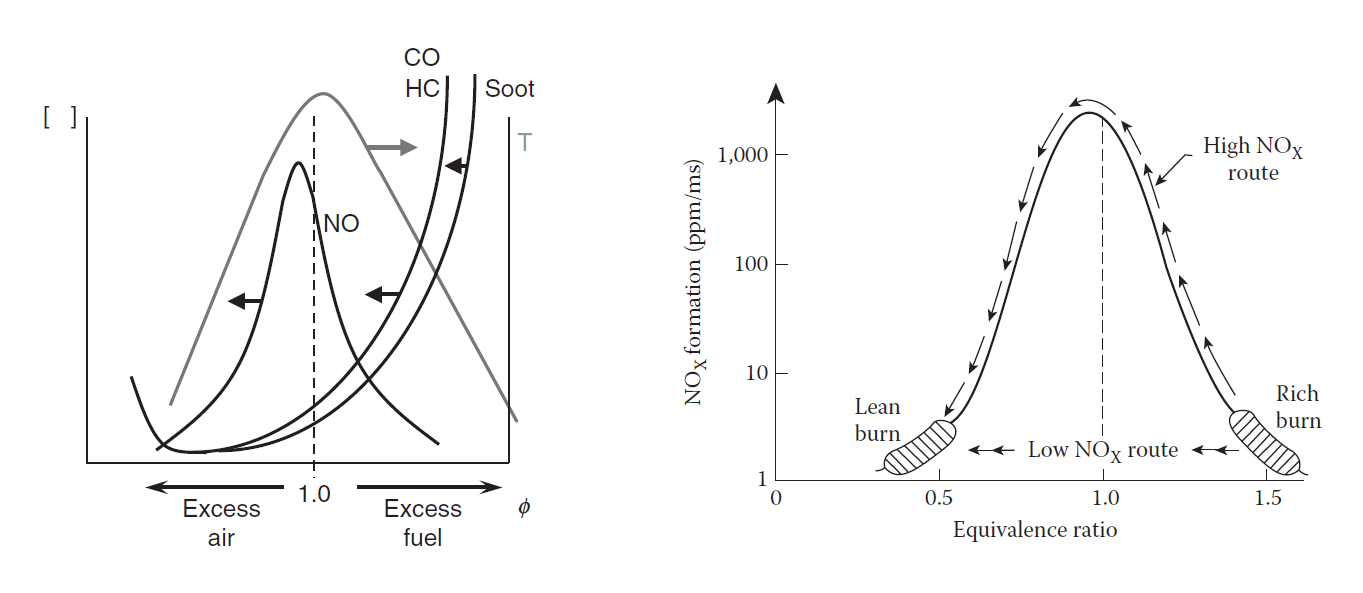
\includegraphics[scale=0.7]{./part0_intro/NOX_motivation_and_RQL}
	\caption{\textsl{Left}: Temperature and species concentration variation with stoichiometric ratio in combustion chambers. Source: \citeColor[dunn-rankin_lean_2008]. \textsl{Right}: NOx formation in Rich-Burn, Quick-Quench, Lean-Burn (RQL) concepts. Source: \citeColor[lefebvre_gas_2010].}
	\label{fig:NOX_motivation_and_RQL}
\end{figure}







\begin{figure}[h!]
	\centering
	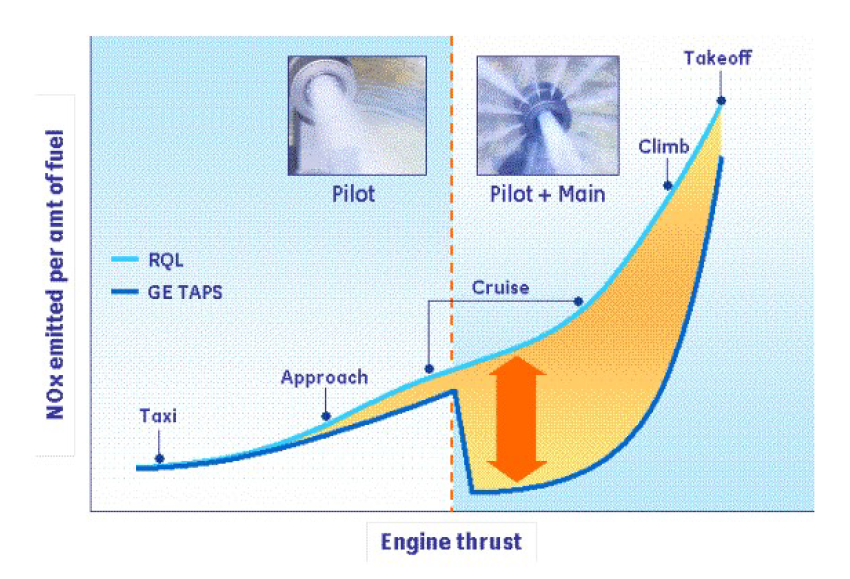
\includegraphics[scale=0.7]{./part0_intro/foust_RQL_vs_TAPS}
	\caption{Source: \citeColor[foust_development_2012].}
	\label{fig:foust_RQL_vs_TAPS}
\end{figure}







\section{Fuel injection technology}

\begin{figure}[h!]
	\centering
	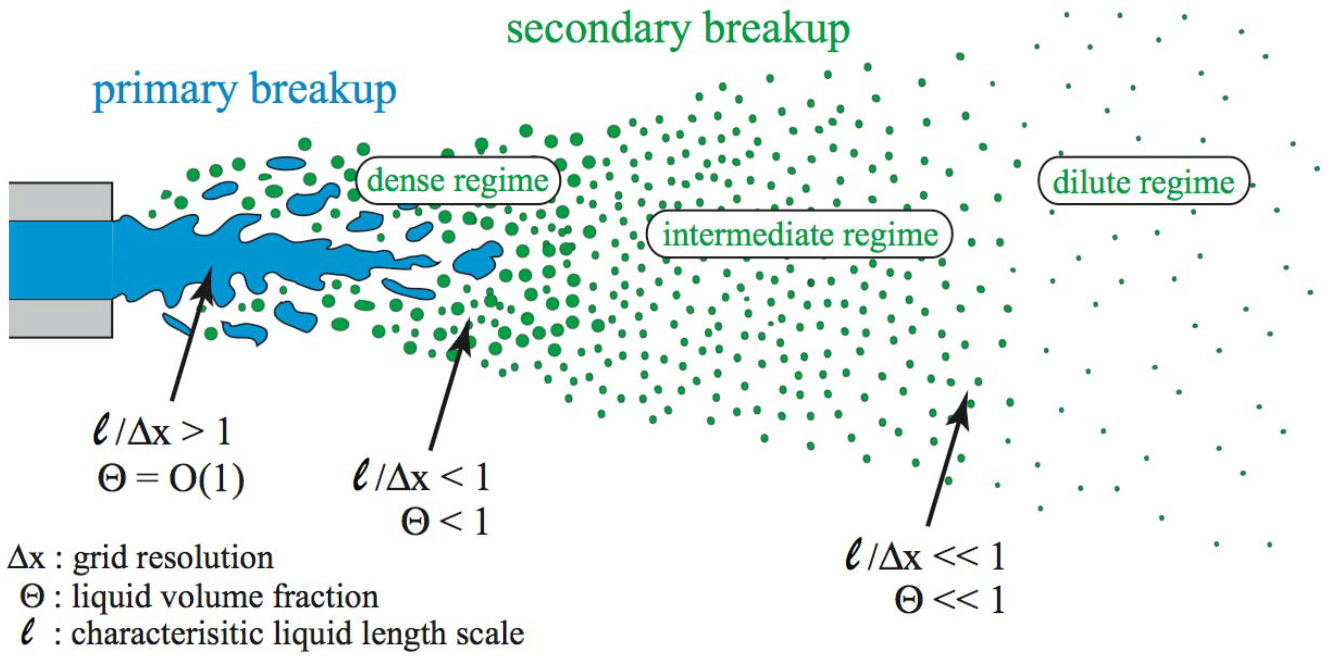
\includegraphics[scale=0.5]{./part0_intro/atomization-regimes-scheme}
	\caption{Atomization breakup regimes \citepColor[herrmann_modeling_2003]}
	\label{fig:atomization_regimes_herrmann}
\end{figure}

\subsection*{Atomization process}

Explain two-phase flows phenomenology (injection + atomization) here. 

Explain airblast, hollow-cone, jicf.

\section{Objective and thesis outline}
    %\addcontentsline{toc}{section}{\protect\numberline{}Manuscript organisation}

